\documentclass[11pt,a4paper]{article}
\usepackage[spanish,es-nodecimaldot]{babel}	% Utilizar español
\usepackage[utf8]{inputenc}					% Caracteres UTF-8
\usepackage{graphicx}						% Imagenes
\usepackage[hidelinks]{hyperref}			% Poner enlaces sin marcarlos en rojo
\usepackage{fancyhdr}						% Modificar encabezados y pies de pagina
\usepackage{float}							% Insertar figuras
\usepackage[textwidth=390pt]{geometry}		% Anchura de la pagina
\usepackage[nottoc]{tocbibind}				% Referencias (no incluir num pagina indice en Indice)
\usepackage{enumitem}						% Permitir enumerate con distintos simbolos
\usepackage[T1]{fontenc}					% Usar textsc en sections
\usepackage{amsmath}						% Símbolos matemáticos

\usepackage[
    backend=biber,
    style=alphabetic,
    sorting=ynt
]{biblatex}                       % Gestion de bibliografia
\addbibresource{mybib.bib}

% Comando para poner el nombre de la asignatura
\newcommand{\asignatura}{Arquitectura y Computación de Altas Prestaciones}
\newcommand{\autor}{Vladislav Nikolov Vasilev}
\newcommand{\titulo}{Trabajo Final de Teoría}
\newcommand{\subtitulo}{Control de Congestión en los Extremos en Comuncaciones
de Granularidad Fina}
\newcommand{\rama}{Ingeniería de Computadores}

% Configuracion de encabezados y pies de pagina
\pagestyle{fancy}
\lhead{\autor{}}
\rhead{\asignatura{}}
\lfoot{Grado en Ingeniería Informática}
\cfoot{}
\rfoot{\thepage}
\renewcommand{\headrulewidth}{0.4pt}		% Linea cabeza de pagina
\renewcommand{\footrulewidth}{0.4pt}		% Linea pie de pagina

\begin{document}
\pagenumbering{gobble}

% Pagina de titulo
\begin{titlepage}

\begin{minipage}{\textwidth}

\centering

%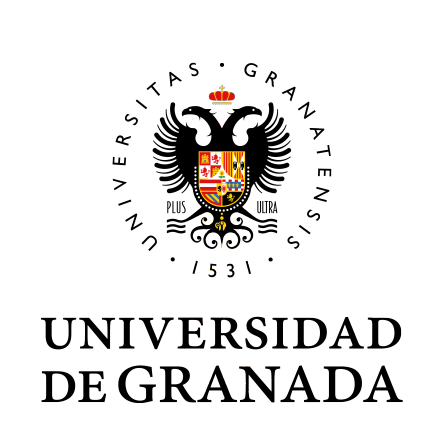
\includegraphics[scale=0.5]{img/ugr.png}\\

\includegraphics[scale=0.3]{img/logo_ugr.jpg}\\[1cm]

\textsc{\Large \asignatura{}\\[0.2cm]}
\textsc{GRADO EN INGENIERÍA INFORMÁTICA}\\[1cm]

\noindent\rule[-1ex]{\textwidth}{1pt}\\[1.5ex]
\textsc{{\Huge \titulo\\[0.5ex]}}
\textsc{{\Large \subtitulo\\}}
\noindent\rule[-1ex]{\textwidth}{2pt}\\[3.5ex]

\end{minipage}

%\vspace{0.5cm}
\vspace{0.7cm}

\begin{minipage}{\textwidth}

\centering

\textbf{Autor}\\ {\autor{}}\\[2.5ex]
\textbf{Rama}\\ {\rama}\\[2.5ex]
\vspace{0.3cm}


\includegraphics[scale=0.3]{img/etsiit.jpeg}

\vspace{0.7cm}
\textsc{Escuela Técnica Superior de Ingenierías Informática y de Telecomunicación}\\
\vspace{1cm}
\textsc{Curso 2019-2020}
\end{minipage}
\end{titlepage}

\pagenumbering{arabic}
\tableofcontents
\thispagestyle{empty}				% No usar estilo en la pagina de indice

\newpage

\setlength{\parskip}{1em}

\section{Introducción}

Las redes en HPC conectan una gran cantidad de nodos, los cuáles se envían
información entre ellos constantemente. Este flujo de información tiene
que ser sin pérdidas, por lo que un fallo en la red o la aparición de congestión
debido a la alta cantidad de tráfico en la red pueden ser un enorme problema.

Según el trabajo, el tráfico de una red puede ser clasificado en dos categorías:

\begin{itemize}[label=\textbullet]
	\item \textbf{Admisible}, si la cantidad de tráfico que se dirige a cada extremos de la red
	no requiere más recursos de los que hay dispnibles. No genera como tal congestión
	en los extremos pero sí que puede llegar a congestionar algún otro punto de la red
	si por ejemplo hay un mal enrutamiento de la información.
	\item \textbf{No admisible}, si la cantidad de tráfico que se dirige a cada extremos de la red
	requiere más recursos de los que hay dispnibles. Este tipo de tráfico produce
	congestión en los extremos.
\end{itemize}

La congestión que aparece en ambos casos causa algo llamado \textit{tree congestion}.
Cuando un nodo tiene su buffer de entrada lleno le indica
a los nodos que le envían información que dejen de enviarle, ya que este no tiene capacidad
para guardar información nueva. Por tanto, la información se comienza a acumular en los buffers 
de entrada de dichos nodos, congestionándolos también y obligándolos a dejar de recibir
nueva información. De esta forma se puede llegar a congestionar y relantizar toda la red
de forma muy rápida si no existe ningún mecanismo de control.

Desde hace algunos años, las GPUs están siendo cada vez más utilizadas en HPC. Esto se traduce
en que se tienen muchas hebras realizando peticiones para acceder a algún recurso compartido
mediante la red. Esto implica tener mucho tráfico donde los mensajes son de poca granularidad.
Esa gran cantidad de tráfico puede llegar a generar congestiones en los extremos, por lo que se
necesitan mecanismos para controlar la congestión causada por dichos mensajes.

\section{Mecanismos existentes para el control de congestión}

Los mecanismos de control de congestión existentes en redes HPC son variados. Algunos de
ellos están basados en software, como por ejemplo sería el caso de los
\textbf{algoritmos de enrutamiento adaptativos}, los cuáles permiten reducir la
\textit{congestión de fábrica} al balancear mejor el tráfico de la red. Otros están
basados en hardware, como es el caso de los protocolos \textbf{ECN} y \textbf{SRP}.

El protocolo ECN (\textit{Explicit Congestion Notification}) se utiliza en conexiones
Infiniband. Cuando se produce congestión en algún punto de la red se notifica mediante
esta conexión y se reduce la cantidad de tráfico que llega a la red (ratio de inyección de
tráfico). Este protocolo funciona bien cuando la congestión es duradera, pero tiene el
principal problema de que espera a que se produzca la congestión para poder notificarla,
controlando por tanto la congestión de forma reactiva.

El protocolo SRP (\textit{Speculative Reservation Protocol}) intenta prevenir la congestión
en los extremos proactivamente. En este protocolo se envía primero un paquete que sirve
para reservar el camino indicando la cantidad de paquetes que se van a mandar, asegurándose
de esta forma que no hay congestión en el extremo. La reserva viaja por un canal de alta
prioridad, y cuando llega al destino se devuelve como respuesta un tiempo de transmisión $t_s$.
Enviado la reserva y sin esperar a la respuesta se empiezan a enviar los otros paquetes de forma
especulativa, viajando estos por un canal virtual de baja prioridad y pudiendo ser descartados
en caso de congestión. Si un paquete especulativo llega al destino correctamente se devuelve
un \texttt{ACK}, y si es descartado por el camino debido a la congestión se devuelve un
\texttt{NACK}. Cuando se recibe un \texttt{NACK} o la respuesta de la reserva se espera el tiempo
indicado por $t_s$ y se mandan los paquetes en modo no especulativo, reenviando en el proceso
aquellos que se han descartado. Estos paquetes viajan por un canal virtual de alta prioridad,
evitando por tanto los posibles retrasos en colas en caso de que exista congestión.

Este segundo protocolo funciona muy bien para controlar la congestión
en caso de que se envíen paquetes grandes. Sin embargo, no funciona demasiado bien con paquetes
pequeños. Esto se debe a que los paquetes de reserva ocupan la mayor parte de los recursos de
la red si los comparamos con los mensajes enviados, los cuáles son pequeños y no requieren tantos
recursos. Por tanto, el mecanismos de reserva por sí mismo reduce el rendimiento de la red al
dejar menos recursos para los paquetes de datos.

\section{Nuevas propuestas de control de congestión}

Para evitar la congestión en los extremos cuando se envían mensajes pequeños se necesitan por
tanto protocolos proactivos (evitan activamente la congestión), rápidos y que no produzcan
una sobrecarga excesiva en la red. En el trabajo se proponen dos nuevos protocolos, los cuáles
se inspiran en el funcionamiento del SRP: el protocolo \textbf{SMSRP} y el protocolo
\textbf{LHRP}.

\subsection{SMSRP}

Las siglas provienen de
\textit{Small-Message Speculative Reservation Protocol}.
Es una modificación directa del protocolo SRP.

Los autores se dieron cuenta que no es necesario hacer siempre una reserva ya que el extremo
puede no sufrir de congestión. Por tanto, solo sería necesario realizarla en los casos en los
que se detecta una congestión en el extremo. Para ello basta
con reordenar el orden de envío del paquete de reconocimiento y de los paquetes especulativos.
Primero se envía el mensaje en modo especulativo y cuando se recibe un \texttt{NACK} se envía un
paquete de reserva. Cuando se recibe la respuesta se espera hasta el tiempo $t_2$ indicado y se
mandan el resto de paquetes y el que se ha descartado en modo no especulativo.

Su principal ventaja es que, teniendo el protocolo SRP implementado en hardware, es muy fácil
implementar este, ya que basta con reordenar el orden en el que se envían los paquetes
especulativos y el reconocimiento. Sin embargo sigue teniendo el mismo problema que el SRP,
que son los mensajes de reserva. Estos pueden llegar a contribuir a la congestión en el extremo
ya que si compiten con los paquetes especulativos van a provocar que estos sean descartados, lo
cuál a su vez va a causar que se envíen más mensajes de reserva, produciéndose por tanto
una sobrecarga de la red.

\subsection{LHRP}

Las siglas provienen de \textit{Last-Hop Reservation Protocol}. Respecto al anterior cambian
algunos aspectos:

\begin{itemize}
	\item En este caso es el último nodo/switch antes del extremo el encargado de las reservas.
	De esta forma se libera al extremo de realizar dicha tarea.
	\item En la misma línea que el punto anterior, se eliminan los mensajes de reserva enviados
	por el origen. Ahora simplemente se pasa de mandar los paquetes en modo especulativo
	a no especulativo cuando se recibe un \texttt{NACK}, esperando obviamente al tiempo $t_2$.
	\item Solo el último switch antes del extremo puede descartar los paquetes especulativos.
	\item Para hacer el control de congestión se añade en el último switch un umbral del
	número de paquetes que pueden estar en la cola. Cuando se excede el umbral, se empiezan
	a descartar los nuevos paquetes que lleguen, obligando a mandarlos en modo no especulativo.	
	De esta forma se evita la aparición de congestión de árbol, ya que se evita que
	se congestionen los nodos anteriores al último switch.
\end{itemize}

\section{Experimentación y resultados}

Los autores han realizado una serie de experimentos en un simulador utilizando una red
\textit{Dragonfly} de 1056 nodos para ver qué tal funcionaban los nuevos protocolos comparándolos
con los existentes y con una red sin mecanismos de control de congestión. Los mensajes enviados
eran de 4 flits.

Primero probaron con una red donde 60 nodos elegidos aleatoriamente mandaban mensajes a 4 nodos
destino mientras los otros permanecían ociosos. De esta forma se pudo simular una red en la
que se pueden llegar a congestionar los extremos debido al constante tráfico. En función de
la cantidad de tráfico se pudieron ver dos cosas:

\begin{enumerate}
	\item LHRP apenas generaba latencia de red pasado el punto de saturación, de forma
	que casi no se produce congestión de ningún tipo en la red. SMSRP tiene una latencia de
	red algo mayor que LHRP a medida que va aumentando el tráfico pasado el punto de
	saturación debido a que se empiezan a descartar más mensajes especulativos y se envían
	más mensajes de reserva, lo cuál sobrecarga ligeramente la red. A pesar
	de eso, son los protocolos que mejores resultados han obtenido si los comparamos con ECN,
	SRP y una red sin control de congestión.
	\item Pasado el punto de saturación, LHRP no genera sobrecarga en la red, de forma que casi
	la totalidad de los mensajes que viajan por la red son de datos, al igual que ocurre en una
	red sin control de congestión. ECN está cerca de este nivel. En el caso de SRP, a partir
	de dicho punto el 30\% del tráfico es de mensajes de reserva. A medida que va aumentando
	el tráfico, el comportamiento del protocolo SMSRP empieza a parecerse al de SRP, ya que
	cada vez habrá más mensajes de reserva viajando por la red.	
\end{enumerate}

Después se hicieron pruebas inyectando en la red tráfico repentino, como si fuesen ráfagas
de tráfico. Aquí se pudo ver que en el caso de los protocolos SMSRP y LHRP la latencia de
los mensajes era pequeña, siendo la latencia del LHRP ligeramente menor que la de SMSRP. Por
tanto, en estos casos se puede afirmar que no se produjo ningún tipo de congestión de la red. Los
otros dos mecanismos probados fueron ECN y la red sin control de congestión. En ellos se
obtuvieron unos peores resultados, pudiéndose apreciar la aparición de congestión.

Finalmente se probó con una red donde no existía congestión con el objetivo de ver qué sobrecarga
generaban los protocolos de control de congestión. Tomando como referencia una red sin control
de congestión, se vio que a medida que aumenta el tráfico las dos propuestas se quedaban
bastante cerda de la red sin control de congestión, indicando por tanto que en líneas generales
producen poca sobrecarga. ECN también se quedaba relativamente cerca, mientras que SRP se quedaba
más atrás, lo cuál implica que es el protocolo que genera una mayor sobrecarga en la red.

\section{Modificaciones sobre las propuestas}

Los autores proponen algunas modificaciones que se pueden hacer sobre el protocolo LHRP:

\begin{itemize}
	\item Se puede modificar el protocolo para que los mensajes se descarten en otros
	puntos que no sean el switch final. De esta forma, el rendimiento mejora si se
	da el caso en el que hay mucha congestión en el extremo.
	\item Se ha visto que el protocolo LHRP base no funciona muy bien para mensajes
	grandes. Por tanto, se podría aumentar el umbral de la cola en el último switch,
	o incluso mejor, se puede combinar con SRP, el cuál sí que funciona bien para mensajes
	grandes, y en función del tamaño del mensaje usar uno u otro. Esto último ha demostrado
	ser bastante eficaz, ya que se genera muy poca latencia extra.
	\item Se puede combinar LHRP con algoritmos de enrutamiento adaptativo para reducir
	la congestión de fábrica con buenos resultados.
\end{itemize}

\section{Conclusiones}

El control de congestión en los extremos para mensajes pequeños ha demostrado ser todo
un reto, ya que requiere de métodos que causen muy poca sobrecarga de red y que sean
capaces de reaccionar rápidamente y de forma proactiva. Los autores propusieron
dos nuevos protocolos, SMSRP y LHRP, los cuáles han ofrecido unos buenos resultados en general,
siendo LHRP mejor en la mayoría de casos, además de producir muy poca o casi ninguna
sobrecarga sobre la red. Aparte de eso, si en una misma red se van a enviar
tanto mensajes pequeños como grandes, se puede combinar LHRP con SRP y elegir uno u otro
en función del tamaño del mensaje.

\newpage

\nocite{*}
\printbibliography[heading=bibintoc]

\end{document}

